% 2026-03-31_vorverstorbenes_kind.tex
% lualatex 2026-03-31_vorverstorbenes_kind.tex
% dvisvgm --no-fonts 2026-03-31_vorverstorbenes_kind.dvi

\documentclass[tikz,border=10pt]{standalone}
\usepackage[T1]{fontenc}
\usepackage{lmodern}
\renewcommand{\familydefault}{\sfdefault}
\usepackage{amsmath}

\usetikzlibrary{positioning, calc}

\begin{document}
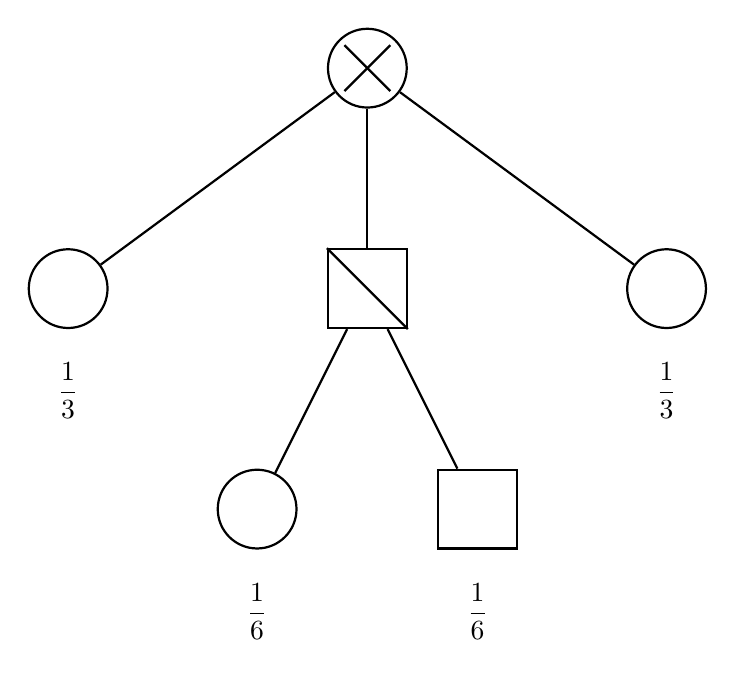
\begin{tikzpicture}[
  thick,
  every node/.style={draw=black, thick},
  level distance=2.8cm,
  level 1/.style={sibling distance=3.8cm},
  level 2/.style={sibling distance=2.8cm},
  edge from parent/.style={draw=black, thick, -},
  grow=down
]

  % Wurzel: Kreis mit X (vorverstorben)
  \node[circle, minimum size=1cm] (root) {}
    child {
      % Linkes Kind: normaler Kreis
      node[circle, minimum size=1cm] (L) {}
      edge from parent
    }
    child {
      % Mittleres Kind: Rechteck mit Diagonale (vorverstorben)
      node[rectangle, minimum size=1cm] (M) {}
      child {
        node[circle, minimum size=1cm] (ML) {}
        edge from parent
      }
      child {
        node[rectangle, minimum size=1cm] (MR) {}
        edge from parent
      }
      edge from parent
    }
    child {
      % Rechtes Kind: normaler Kreis
      node[circle, minimum size=1cm] (R) {}
      edge from parent
    };

  % X durch die Wurzel zeichnen
  \draw ($(root.north west)!0.1!(root.south east)$)
     -- ($(root.north west)!0.9!(root.south east)$);
  \draw ($(root.north east)!0.1!(root.south west)$)
     -- ($(root.north east)!0.9!(root.south west)$);

  % Diagonale durch mittleres Kind (Ebene 1)
  \draw (M.north west) -- (M.south east);

  % Brüche unterhalb Ebene 1
  \node[draw=none, below=0.3cm of L,  font=\sffamily] {$\dfrac{1}{3}$};
  \node[draw=none, below=0.3cm of R,  font=\sffamily] {$\dfrac{1}{3}$};

  % Brüche unterhalb Ebene 2
  \node[draw=none, below=0.3cm of ML, font=\sffamily] {$\dfrac{1}{6}$};
  \node[draw=none, below=0.3cm of MR, font=\sffamily] {$\dfrac{1}{6}$};

\end{tikzpicture}
\end{document}